\documentclass[12pt,a4paper,fontset=none]{ctexart}

\usepackage[a4paper,top=2.6cm,bottom=2.6cm,left=2.6cm,right=2.6cm]{geometry}
\usepackage{xeCJK}
\setCJKmainfont{Songti}[Path=/System/Library/Fonts/Supplemental/,Extension=.ttc]
\setCJKfamilyfont{zhhei}{STHeiti Medium}[Path=/System/Library/Fonts/,Extension=.ttc]
\setCJKfamilyfont{zhkai}{楷体_GB2312}[Path=/Users/kinakoxu/Library/Fonts/,Extension=.ttf]
\setCJKfamilyfont{zhfs}{仿宋_GB2312}[Path=/Users/kinakoxu/Library/Fonts/,Extension=.ttf]
\newcommand{\heiti}{\CJKfamily{zhhei}}
\newcommand{\kaishu}{\CJKfamily{zhkai}}
\newcommand{\fangsong}{\CJKfamily{zhfs}}

\usepackage{graphicx}
\usepackage{booktabs}
\usepackage{amsmath}
\usepackage{hyperref}
\usepackage{float}
\usepackage{xcolor}
\usepackage{listings}
\usepackage{longtable}
\usepackage{array}
\usepackage{caption}
\usepackage{setspace}
\usepackage{enumitem}

\hypersetup{colorlinks=true,linkcolor=black,urlcolor=blue,citecolor=black}
\setstretch{1.3}
\setlength{\parindent}{2em}
\setlength{\parskip}{0.2em}

\captionsetup{font=small,labelsep=space}

\lstset{
  language=Python,
  basicstyle=\ttfamily\small,
  keywordstyle=\color{blue!70!black}\bfseries,
  commentstyle=\color{teal!60!black},
  stringstyle=\color{brown!70!black},
  numbers=left,
  numberstyle=\scriptsize\color{gray},
  stepnumber=1,
  numbersep=8pt,
  frame=single,
  breaklines=true,
  showstringspaces=false,
  tabsize=4,
  backgroundcolor=\color{gray!5},
  xleftmargin=1.5em,
  xrightmargin=0.5em,
  aboveskip=0.8em,
  belowskip=0.8em
}

\title{
  \vspace*{2cm}
  
\includegraphics[width=0.18\textwidth]{../TongjiThesis-master/figures/tongji.pdf}\\[1em]
  {\heiti\zihao{-1}同济大学}\\[0.4em]
  {\bfseries\Large TONGJI UNIVERSITY}\\[2.5em]
  {\heiti\zihao{-2}机器人避障\\寻径问题}
}
\author{}
\date{}

\begin{document}

\maketitle
\thispagestyle{empty}

\begin{center}
\renewcommand{\arraystretch}{1.9}
\begin{tabular}{p{4.5em}p{16em}}
学院 & 国豪书院 \\
姓名 & 徐佳涛 \\
学号 & 2452627 \\
老师 & 张红云 \\
\end{tabular}
\end{center}

\clearpage
\tableofcontents
\clearpage

\section{问题背景与动态场景建模}

机器人避障寻径问题的目标是在存在障碍物的环境中，为机器人规划一条从起点到终点的无碰撞路径。这个问题既可以看成图搜索问题，也可以看成智能体在环境中的决策问题，因此很适合用来比较传统搜索算法和强化学习方法的差异。

本次课程设计以二维栅格地图为研究对象。地图中的网格只分为空地和障碍，机器人每一步只能向上、下、左、右四个方向移动。课程要求先完成基础的 A* 与 BFS 算法，再进一步设计更高难度的场景，并尝试加入其他算法进行改进。

本文在原始 9$\times$8 基础场景外，又设计了一个 30$\times$30 的复杂场景。该场景通过长墙、窄门、U 型障碍和假通路增加搜索难度，从而更容易观察不同算法在搜索效率、路径质量和鲁棒性上的差异。另一方面，在动态展示部分，地图状态会随着搜索过程逐帧更新，因此也体现了“动态场景建模”的要求。

\begin{lstlisting}[caption={30x30 场景图的构造方式}]
def get_challenge_map(size=30):
    grid = np.zeros((size, size), dtype=int)
    grid[0, :] = 1
    grid[-1, :] = 1
    grid[:, 0] = 1
    grid[:, -1] = 1

    for col, rows in vertical_walls.items():
        for row in rows:
            grid[row, col] = 1
\end{lstlisting}

\section{项目结构与程序设计}

本次课程设计的核心程序文件包括：
\begin{itemize}[nosep]
  \item \texttt{pathfinder.py}：主程序，负责 BFS、A*、改进 A*、Q-Learning、人工势场法的统一实验；
  \item \texttt{Dijikstra.py}：单独实现 Dijkstra 算法，并与 BFS、A* 进行对比；
  \item 实验结果图与 GIF 文件：用于静态对比和动态展示。
\end{itemize}

整体程序流程可以概括为“建图、搜索、统计、绘图”四个步骤。主程序先创建地图，再调用不同算法进行寻路，随后输出访问节点数、路径步数和综合代价，最后生成结果图和动态图。

\begin{lstlisting}[caption={主程序的整体流程}]
def main():
    basic_grid, basic_start, basic_end = get_basic_map()
    basic_results = compare_on_map(basic_grid, basic_start, basic_end)

    challenge_grid, challenge_start, challenge_end = get_challenge_map()
    challenge_results = compare_on_map(
        challenge_grid, challenge_start, challenge_end
    )
\end{lstlisting}

\section{算法设计}

\subsection{BFS 算法}

广度优先搜索（BFS）按照层次逐层扩展节点。在单位代价栅格地图中，BFS 能保证第一次到达终点时得到最短路径。它的优点是实现简单、结果稳定；缺点是搜索盲目性较强，在复杂场景中会访问大量无关节点。

\subsection{A* 算法}

A* 在一致代价搜索基础上加入启发式函数，评价函数定义为
\begin{equation}
f(n)=g(n)+h(n),
\end{equation}
其中 $g(n)$ 表示起点到当前节点的实际代价，$h(n)$ 表示当前节点到终点的估计代价。本文使用曼哈顿距离作为启发式函数，因此 A* 在相同路径长度下通常比 BFS 访问更少的节点。

\subsection{改进 A* 算法}

基础 A* 只关注路径长度，不考虑路径是否贴近障碍，也不考虑转弯是否过多。为此，本文在单步代价中加入贴障惩罚和转向惩罚，使得搜索结果更平滑，也更符合机器人真实运动需求。

\subsection{Q-Learning 算法}

Q-Learning 属于强化学习方法。它通过环境反馈不断更新状态-动作价值函数，从而逐渐学会从起点移动到终点的策略。相比图搜索算法，它具有学习能力；但训练过程更长，且效果比较依赖奖励函数设计。

\subsection{人工势场法}

人工势场法把目标看作吸引源，把障碍物看作排斥源，机器人沿合成势场方向移动。该方法实现简单、局部反应快，但在复杂场景中容易陷入局部极小值。

\subsection{Dijkstra 算法}

Dijkstra 是求解非负权图最短路径的经典方法。在本文的单位代价栅格环境中，它可以看作不带启发式信息的一致代价搜索。它稳定可靠，但在复杂场景中的效率通常低于 A*。

\section{核心代码实现}

\subsection{BFS 核心代码}

\begin{lstlisting}[caption={BFS 的核心实现}]
def bfs_search(grid, start, end):
    queue = deque([start])
    visited = {start}
    came_from = {}

    while queue:
        current = queue.popleft()
        if current == end:
            return reconstruct_path(came_from, current)

        for nxt in get_neighbors(grid, current):
            if nxt not in visited:
                visited.add(nxt)
                came_from[nxt] = current
                queue.append(nxt)
\end{lstlisting}

\subsection{A* 核心代码}

\begin{lstlisting}[caption={A* 的节点扩展逻辑}]
def a_star_search(grid, start, end):
    open_set = []
    heapq.heappush(open_set, (0, start))
    g_score = {start: 0}

    while open_set:
        _, current = heapq.heappop(open_set)
        if current == end:
            return True

        for nxt in get_neighbors(grid, current):
            tentative_g = g_score[current] + 1
            heuristic = abs(nxt[0] - end[0]) + abs(nxt[1] - end[1])
            f_score = tentative_g + heuristic
            heapq.heappush(open_set, (f_score, nxt))
\end{lstlisting}

\subsection{改进 A* 核心代码}

\begin{lstlisting}[caption={改进 A* 的附加代价}]
step_cost = 1.0
step_cost += nearby_obstacle_penalty(grid, nxt)
if prev_dir is not None and direction != prev_dir:
    step_cost += 0.1

heuristic = manhattan(nxt, end)
heuristic += 0.2 * nearby_obstacle_penalty(grid, nxt)
f_score = tentative_g + heuristic_weight * heuristic
\end{lstlisting}

\subsection{Q-Learning 核心代码}

\begin{lstlisting}[caption={Q-Learning 的价值更新}]
reward = self.step_reward(state, nxt, valid, seen)
best_next = np.max(self.q_table[nxt[0], nxt[1]])
td_target = reward + self.gamma * best_next
td_error = td_target - self.q_table[state[0], state[1], action]
self.q_table[state[0], state[1], action] += self.alpha * td_error
\end{lstlisting}

\subsection{Dijkstra 核心代码}

\begin{lstlisting}[caption={Dijkstra 的核心实现}]
priority_queue = [(0.0, start)]
distances = {start: 0.0}

while priority_queue:
    current_cost, current = heapq.heappop(priority_queue)
    if current == end:
        return True
    for neighbor in get_neighbors(grid, current):
        new_cost = current_cost + 1.0
        if new_cost < distances.get(neighbor, float("inf")):
            distances[neighbor] = new_cost
            heapq.heappush(priority_queue, (new_cost, neighbor))
\end{lstlisting}

\section{实验结果与动态可视化}

\subsection{实验环境}

\begin{table}[H]
\centering
\caption{实验环境配置}
\begin{tabular}{ll}
\toprule
项目 & 配置 \\
\midrule
编程语言 & Python 3.13.9 \\
数值计算库 & NumPy 2.3.5 \\
可视化库 & Matplotlib 3.10.6 \\
地图规模 & 9x8 与 30x30 \\
动态展示方式 & 导出 GIF 动画文件 \\
\bottomrule
\end{tabular}
\end{table}

\subsection{基础场景结果}

\begin{table}[H]
\centering
\caption{基础场景实验结果}
\begin{tabular}{lcccc}
\toprule
算法 & 是否成功 & 访问节点数 & 路径步数 & 综合代价 \\
\midrule
BFS & 是 & 57 & 20 & 20.00 \\
A* & 是 & 32 & 20 & 27.20 \\
改进 A* & 是 & 35 & 20 & 26.20 \\
Q-Learning & 是 & 21 & 20 & 27.20 \\
人工势场法 & 否 & 25 & 24 & -- \\
\bottomrule
\end{tabular}
\end{table}

\begin{figure}[H]
\centering
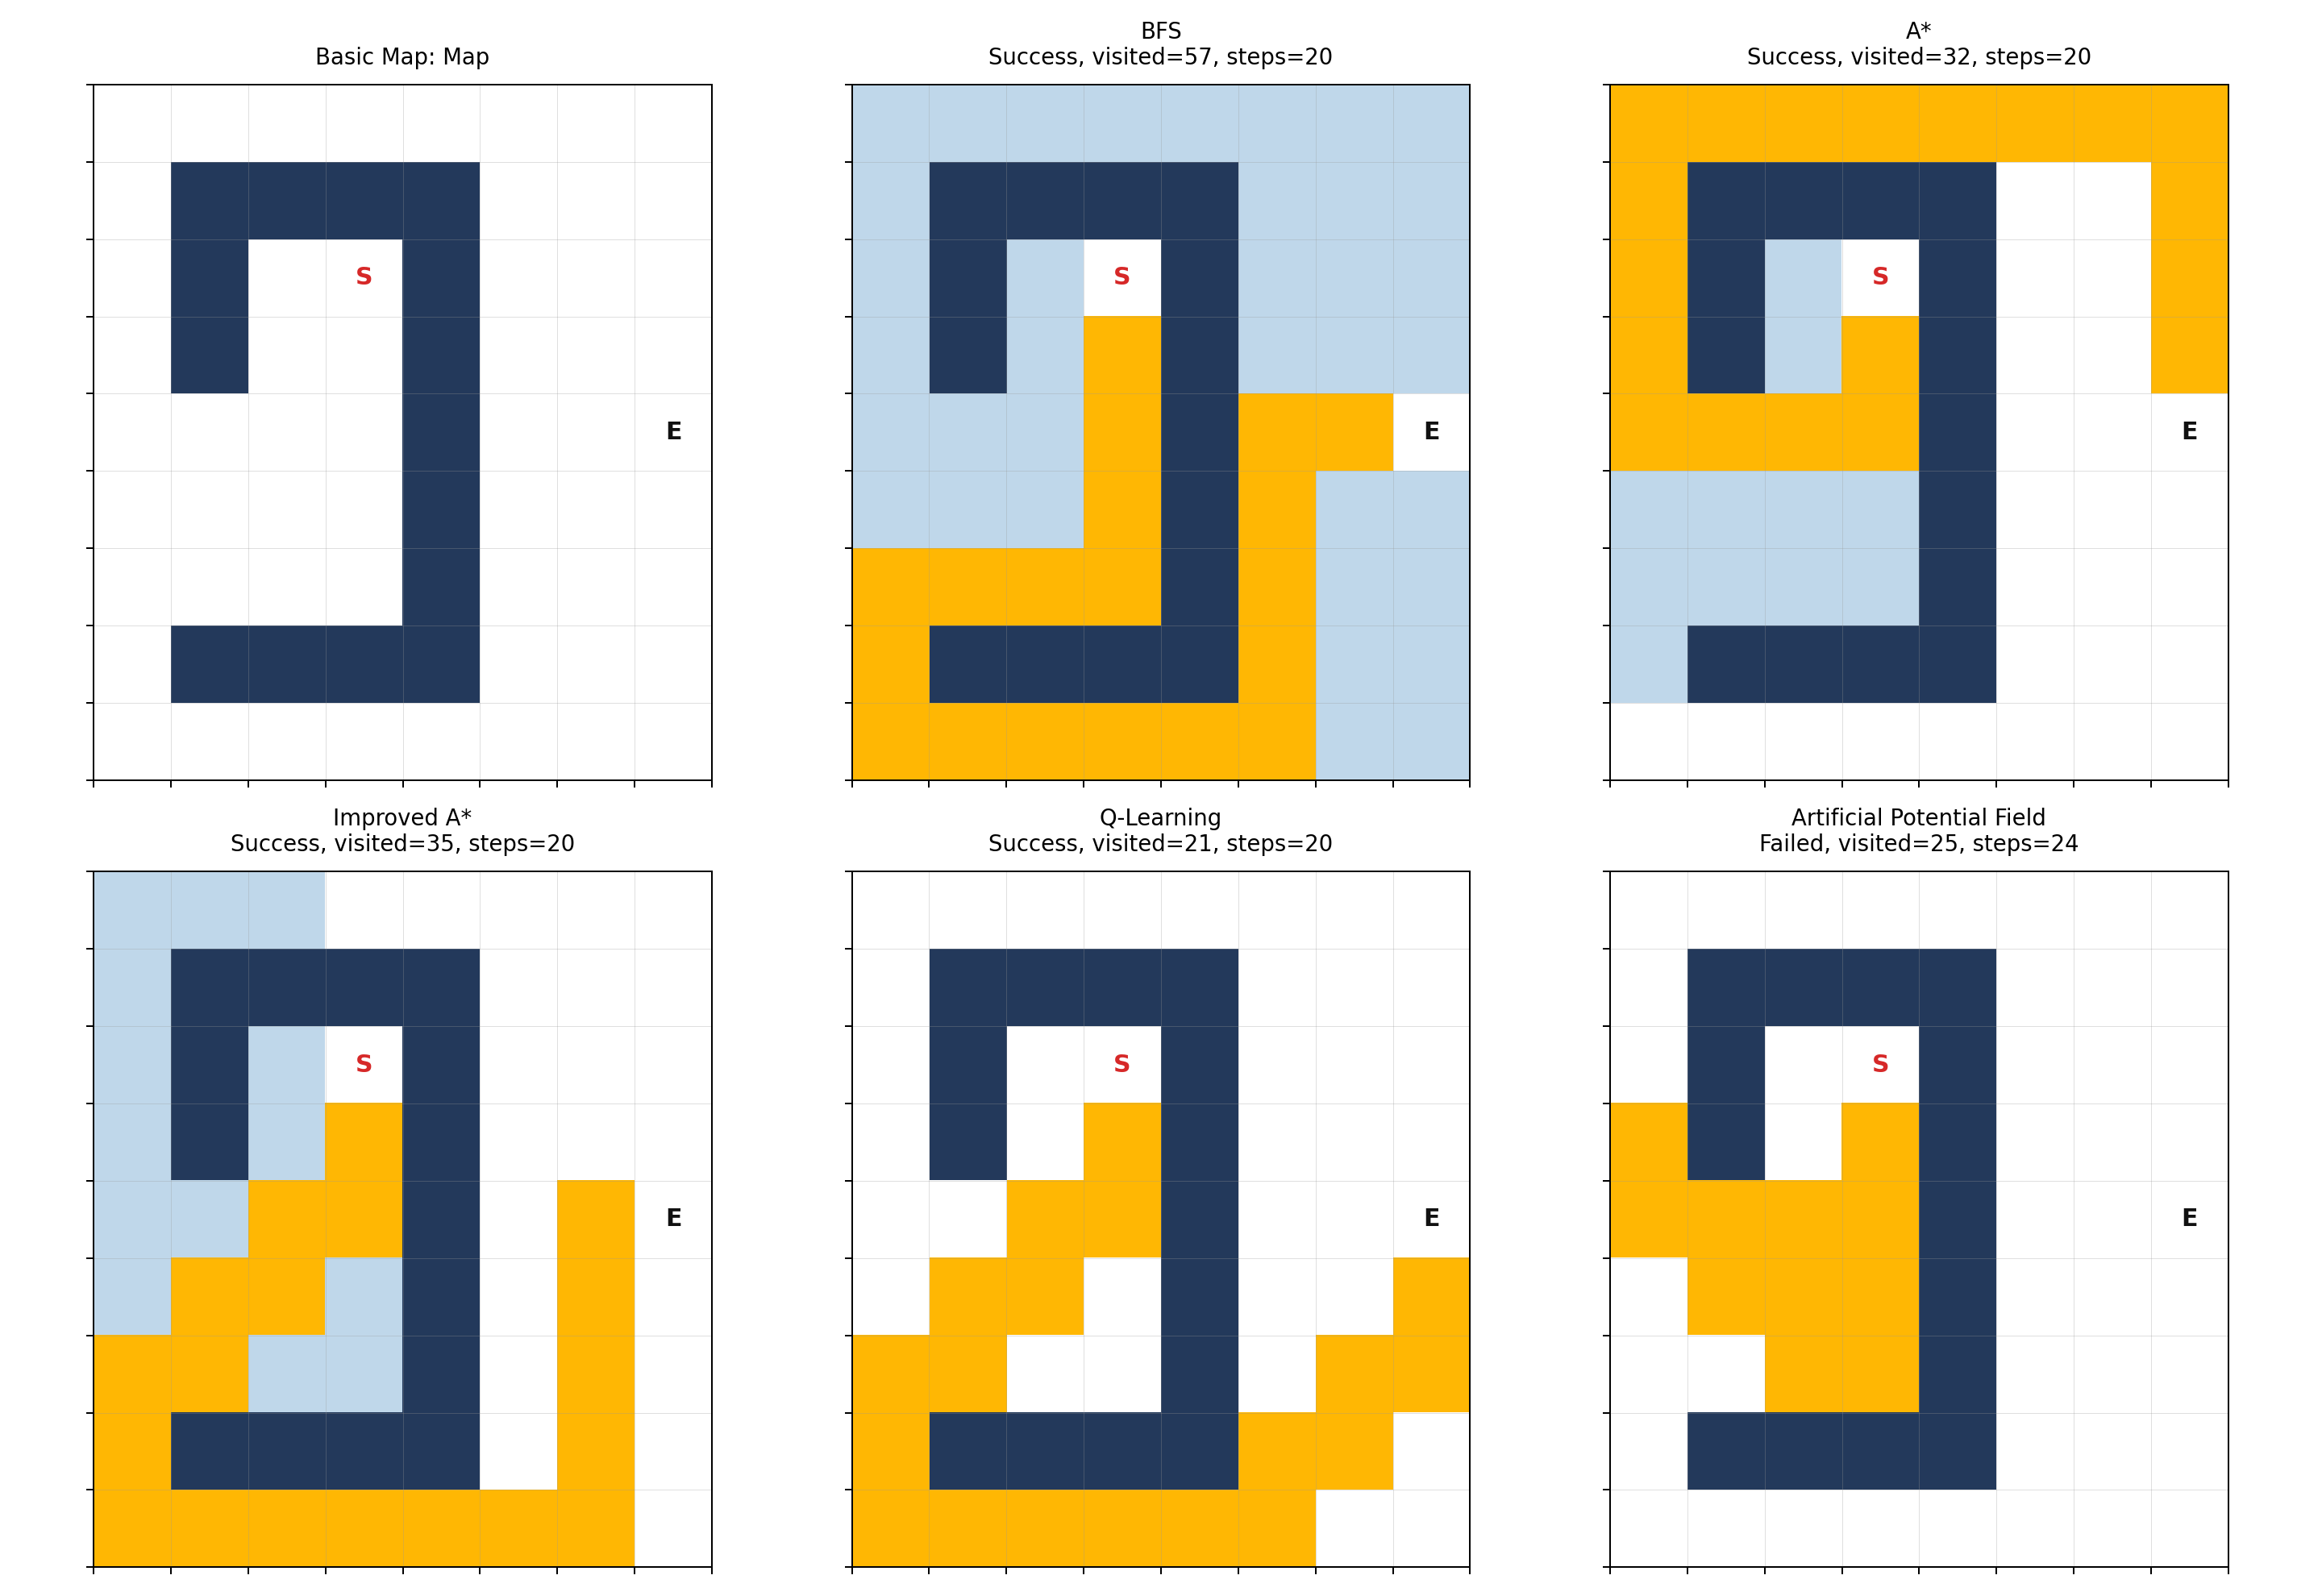
\includegraphics[width=0.82\textwidth]{../basic_map_comparison.png}
\caption{基础场景下各算法结果对比}
\end{figure}

\subsection{复杂场景结果}

\begin{table}[H]
\centering
\caption{30x30 复杂场景实验结果}
\begin{tabular}{lcccc}
\toprule
算法 & 是否成功 & 访问节点数 & 路径步数 & 综合代价 \\
\midrule
BFS & 是 & 334 & 64 & 64.00 \\
Dijkstra & 是 & 334 & 64 & 82.20 \\
A* & 是 & 231 & 64 & 81.96 \\
改进 A* & 是 & 263 & 64 & 79.56 \\
Q-Learning & 是 & 65 & 64 & 81.64 \\
人工势场法 & 否 & 91 & 90 & -- \\
\bottomrule
\end{tabular}
\end{table}

\begin{figure}[H]
\centering
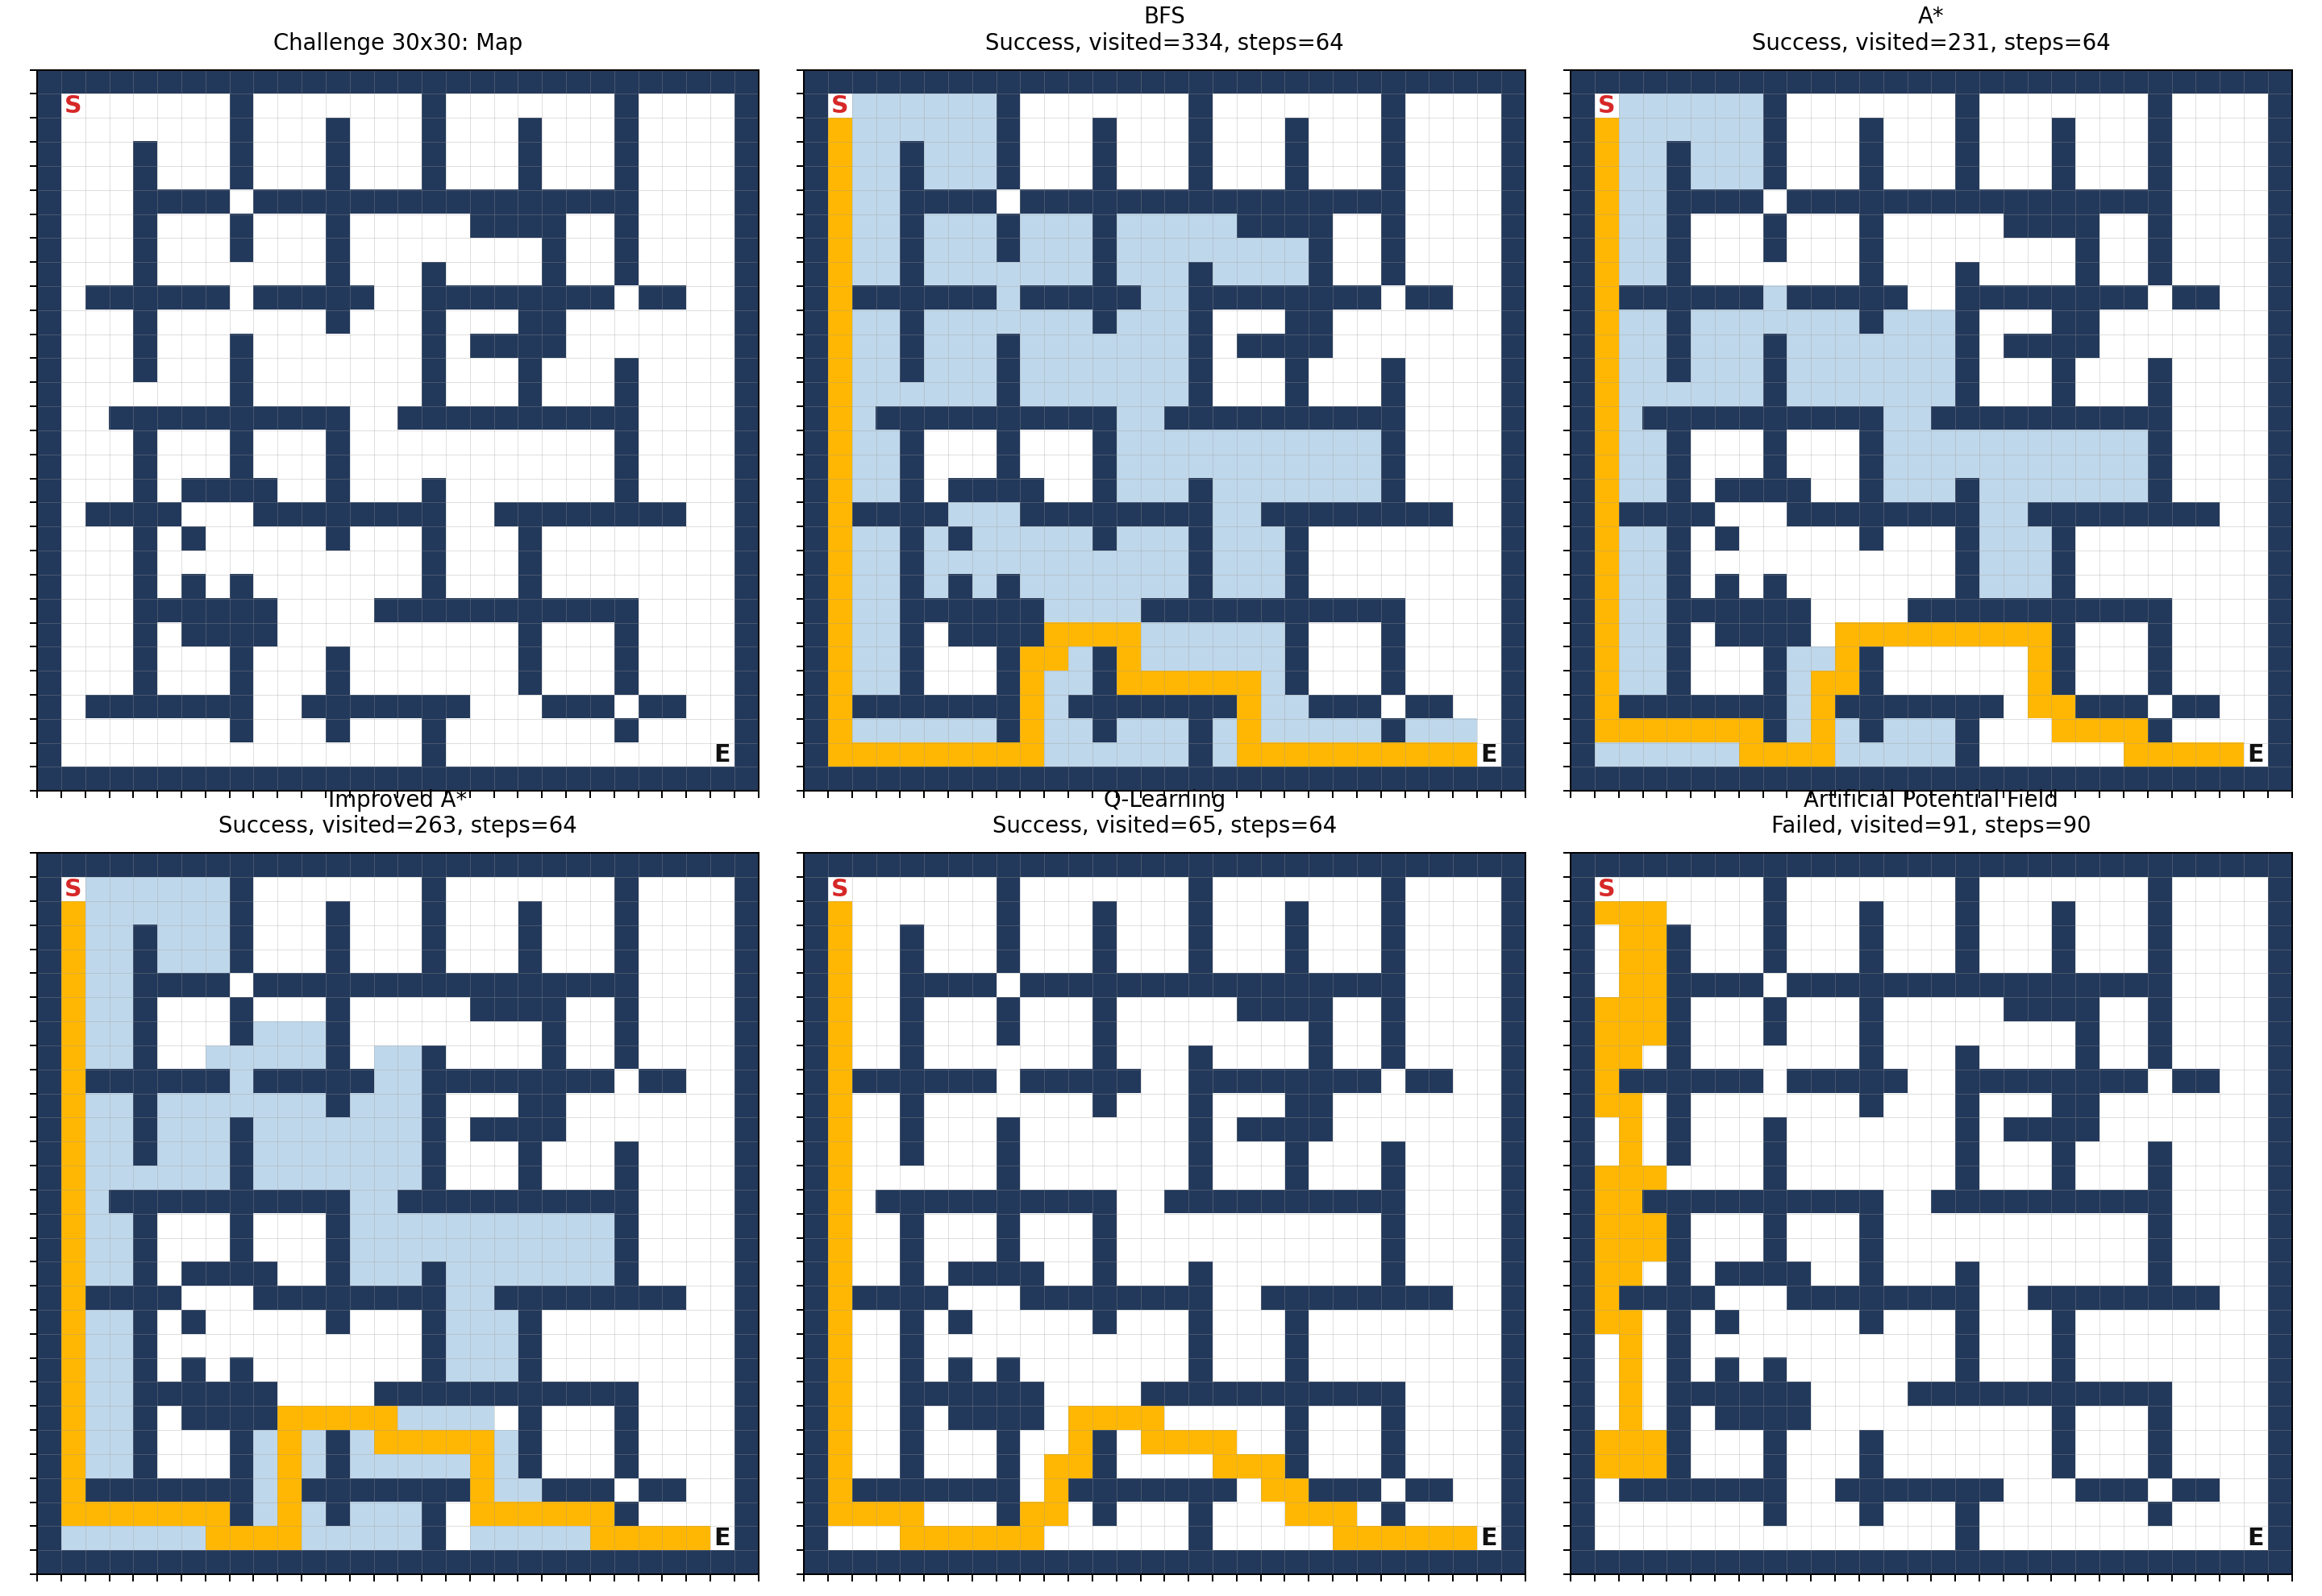
\includegraphics[width=0.9\textwidth]{../challenge_30x30_comparison.png}
\caption{30x30 复杂场景下各算法结果对比}
\end{figure}

\begin{figure}[H]
\centering
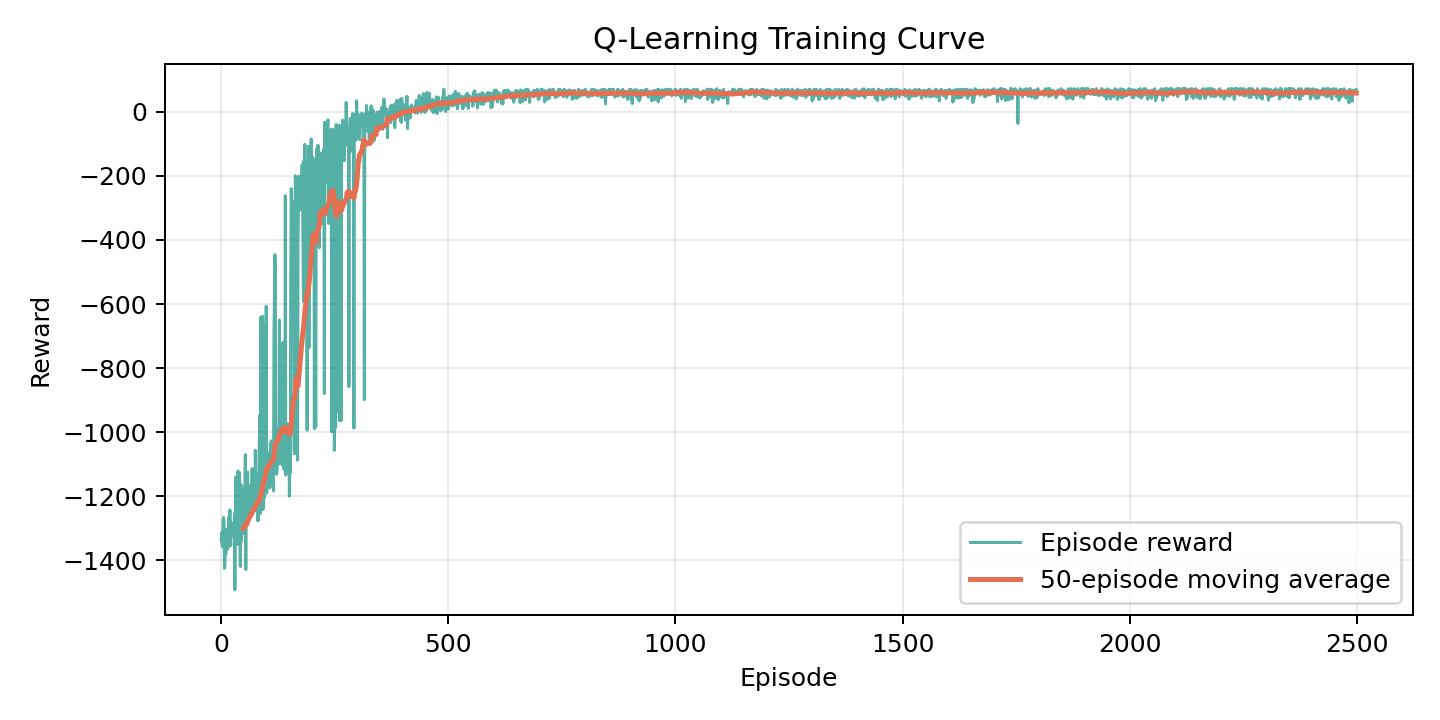
\includegraphics[width=0.7\textwidth]{../challenge_30x30_q_learning_curve.png}
\caption{Q-Learning 在复杂场景中的训练回报曲线}
\end{figure}

\begin{figure}[H]
\centering
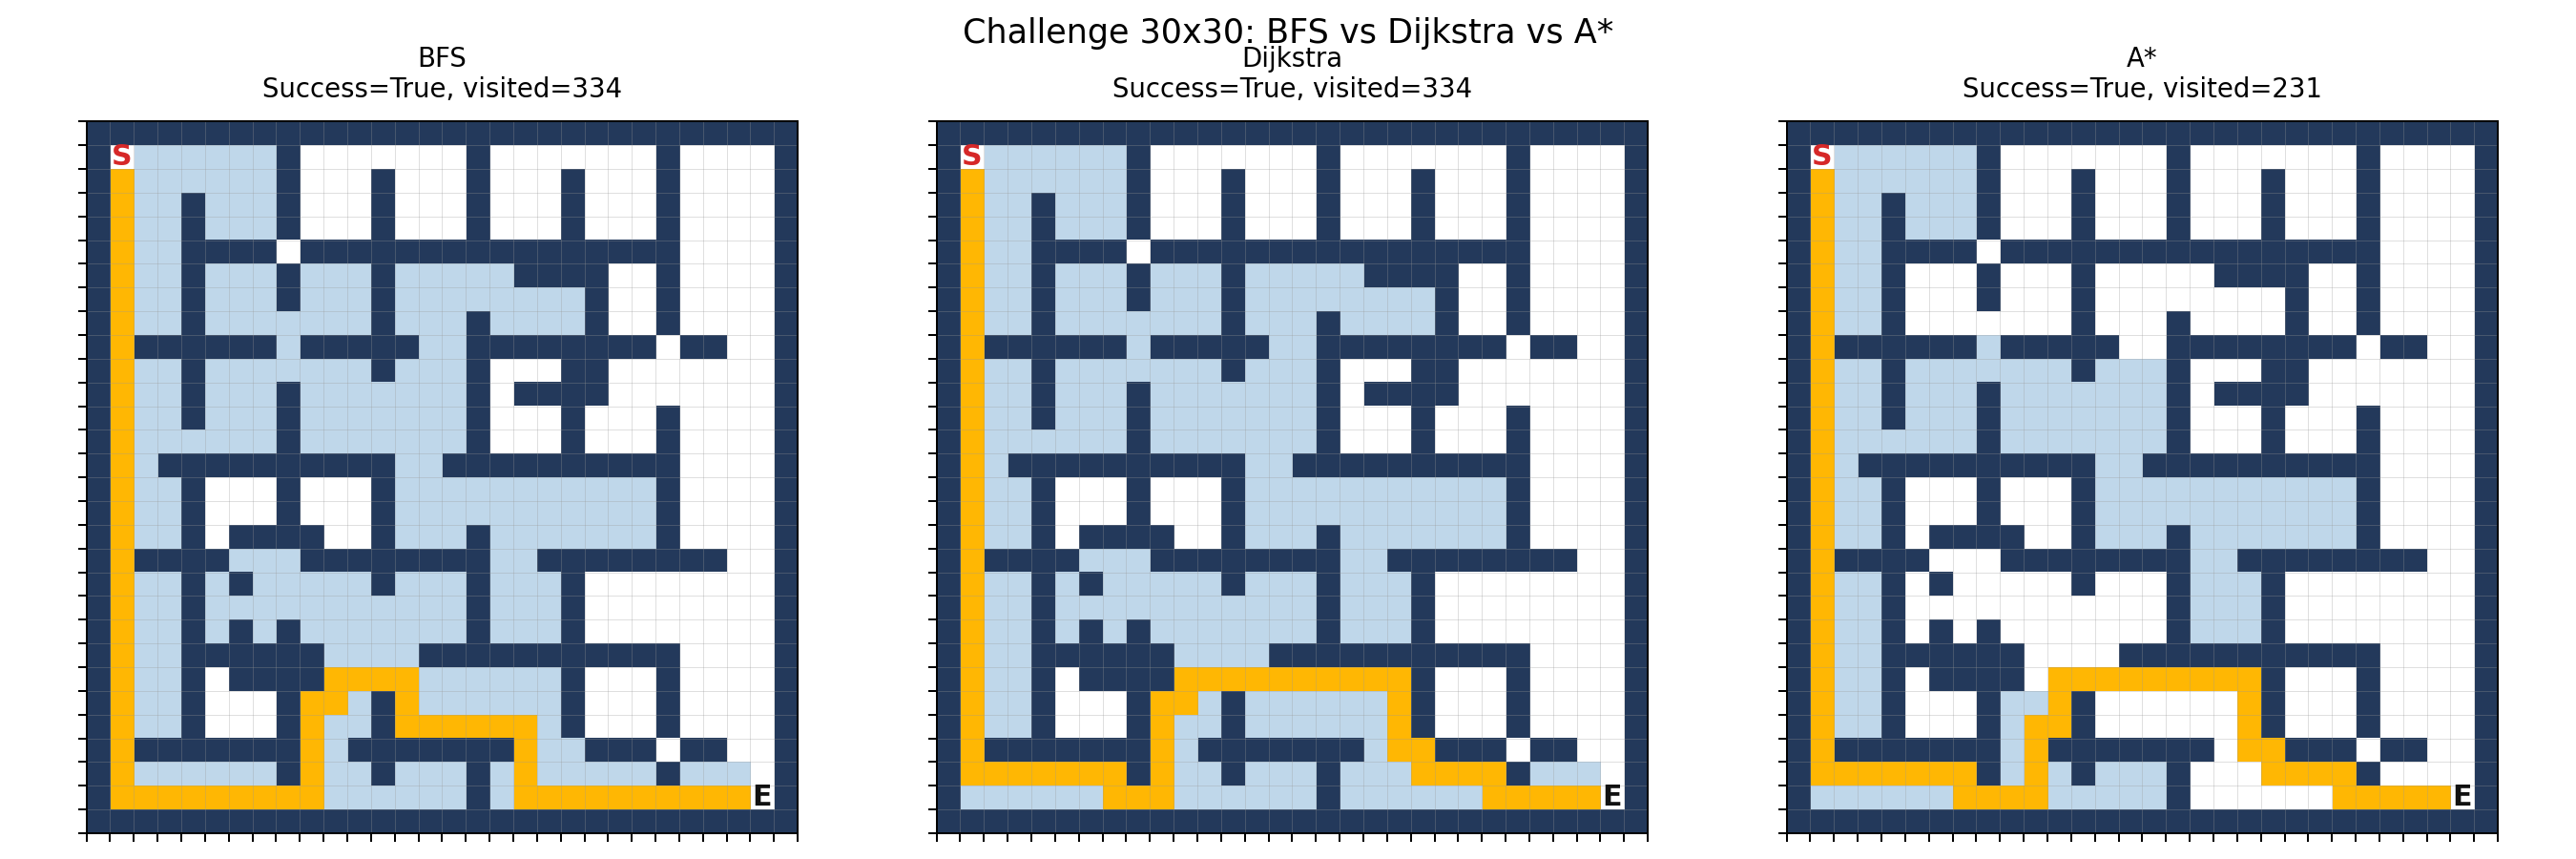
\includegraphics[width=0.75\textwidth]{../dijkstra_challenge_comparison.png}
\caption{BFS、Dijkstra 与 A* 在复杂场景中的对比}
\end{figure}

\subsection{动态可视化}

为了满足题目对动态展示的要求，本文把 BFS、A* 和改进 A* 的搜索过程导出为 GIF 动画。整个动态展示分为两个阶段：第一阶段显示节点访问顺序；第二阶段在到达终点后显示最终路径回溯。通过这些动态图，可以明显看出 BFS 更像“波纹式”扩展，而 A* 的搜索方向更集中。

\begin{lstlisting}[caption={动态展示中的帧更新逻辑}]
def update(frame_idx):
    display = np.copy(base_grid)

    for node in visited_frames[:frame_idx]:
        if node not in (start, end) and display[node] == 0:
            display[node] = 2

    if frame_idx >= len(visited_frames) and result.success:
        path_idx = frame_idx - len(visited_frames)
        for node in path_frames[:path_idx]:
            if node not in (start, end):
                display[node] = 3
\end{lstlisting}

\section{结果分析与讨论}

从实验结果可以看出，BFS 与 Dijkstra 都能够稳定找到最短路径，但在复杂场景中访问节点数很多，说明这两类算法虽然可靠，但搜索效率偏低。A* 在引入启发式函数后，访问节点明显减少，说明启发式信息确实能够有效缩小搜索范围。

改进 A* 的路径长度与普通 A* 一致，但综合代价更低，这说明加入贴障惩罚和转向惩罚后，路径质量得到了提升。虽然它的访问节点数不一定最少，但在“更安全、更平滑”这一目标上表现更好。

在本文的实验中，Dijkstra 是一个很有代表性的对照算法。由于当前栅格地图中每一步的基础移动代价相同，所以 Dijkstra 与 BFS 在“是否能找到最短路径”这一点上表现接近，二者都能够稳定得到最短长度路径。但从搜索过程来看，Dijkstra 仍然需要像 BFS 一样扩展大量节点，因此在复杂场景中的效率不高。

与 A* 相比，Dijkstra 最大的区别在于它不使用终点方向信息。A* 会借助启发式函数优先扩展更接近终点的节点，所以在 30x30 场景中访问节点数明显少于 Dijkstra。这说明在静态已知地图中，启发式信息确实能够有效降低搜索范围。

与改进 A* 相比，Dijkstra 的优点是思路简单、最短路性质明确，不需要额外调参；缺点是无法表达贴障风险和转弯代价这类路径质量信息。改进 A* 虽然不一定在节点数上绝对占优，但生成的路径通常更平滑，也更符合机器人实际运动需求。

Q-Learning 在训练足够轮次后能够成功找到路径，说明强化学习方法在此类问题上具有可行性。相比图搜索算法，它的优势在于可以通过交互学习策略；不足之处在于训练时间较长，而且结果对奖励函数设计比较敏感。

人工势场法在简单环境中表现较直观，但在本文设计的复杂 30x30 场景中出现了失败，原因主要是 U 型障碍和窄通道导致局部极小值问题。这也说明人工势场法更适合作为局部避障方法，而不太适合单独承担复杂场景下的全局规划任务。

当前方案仍然存在一些局限：当前地图是静态已知环境，没有加入动态障碍；机器人运动方式只考虑四个方向，没有考虑速度和转向半径等真实约束；Q-Learning 仍然是表格型实现，状态规模扩大后训练成本会快速增加；动态展示目前以 GIF 形式导出，交互性还不够强。

\section{总结}

本次课程设计围绕机器人避障寻径问题，完成了从基础算法实现、复杂场景设计，到多算法比较和动态可视化展示的一整套实验流程。具体来说，本文首先实现了 BFS 和 A* 两种基础算法；随后自主设计了一个 30x30 的复杂障碍场景；在此基础上补充实现了改进 A*、Q-Learning、人工势场法和 Dijkstra；最后输出了静态结果图、训练曲线和 GIF 动态展示文件。

实验结果表明：BFS 和 Dijkstra 能稳定得到最短路径，但搜索范围较大；A* 具有更高的搜索效率；改进 A* 能在路径长度不变的前提下降低综合代价；Q-Learning 经过训练后能够得到可行路径；人工势场法在复杂环境中容易受到局部极小值影响。整体来看，本次课程设计不仅完成了题目要求，也让我对图搜索算法、强化学习方法以及路径规划中的可视化展示有了更直观的理解。

\end{document}
